\section{Fragmentation}

\pgfdeclareimage[width=1.0\paperwidth]{header-image}{header_images/helicopter}
\againframe<5->{framework}

\controlsSide{limitation_map}{2}{controlMaps}

\begin{frame}
    \frametitle{So Humans have no impact of fire?}
    \framesubtitle{Land use}
    %Start of with increase in burnt area from Igntions
    %Then add in land framgentation
\end{frame}

\pgfdeclareimage[width=1.0\paperwidth]{header-image}{header_images/Mirador_de_Garbi}
\begin{frame}
    \frametitle{So Humans have no impact of fire?}
    \framesubtitle{Fragmentation}
    \begin{textblock*}{11cm}(0.5cm,1.5cm)
    \visible<1-2>{
        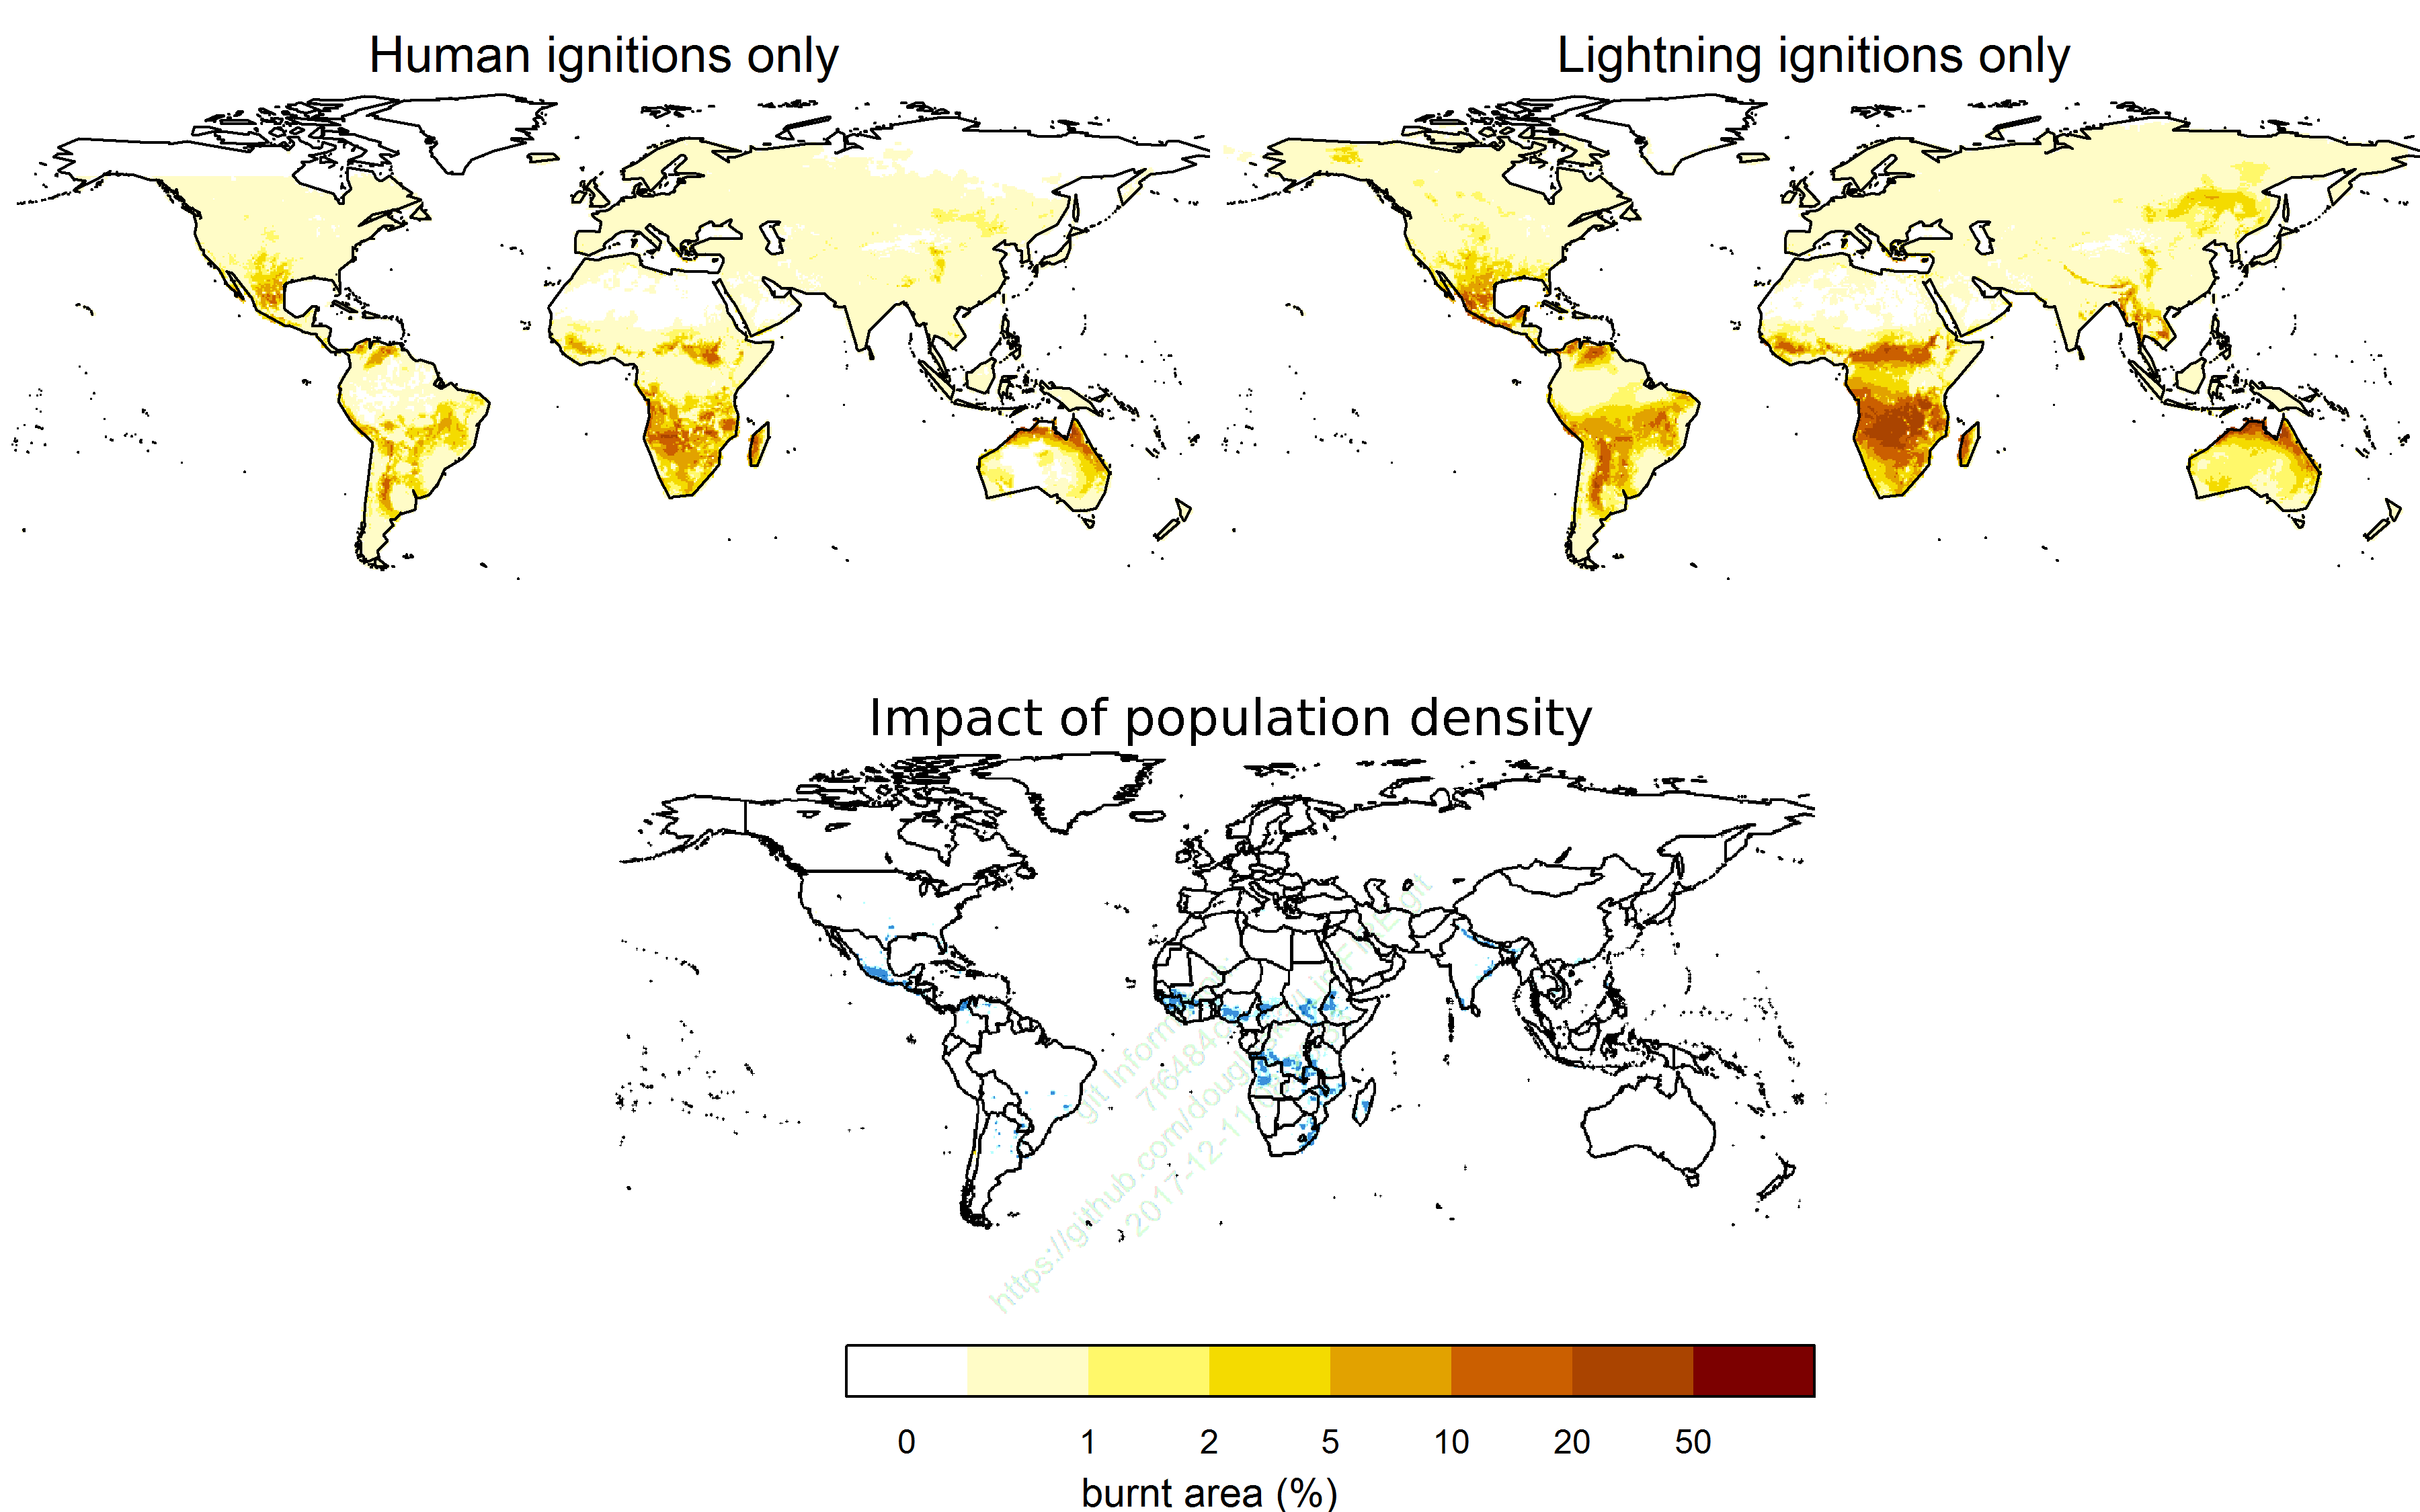
\includegraphics[trim={10.3cm 2cm 0cm 8.44cm},clip,width=6.5cm]{images/igntitions/IgntionInfoSourceAdding}
    }

    \only<2>{
        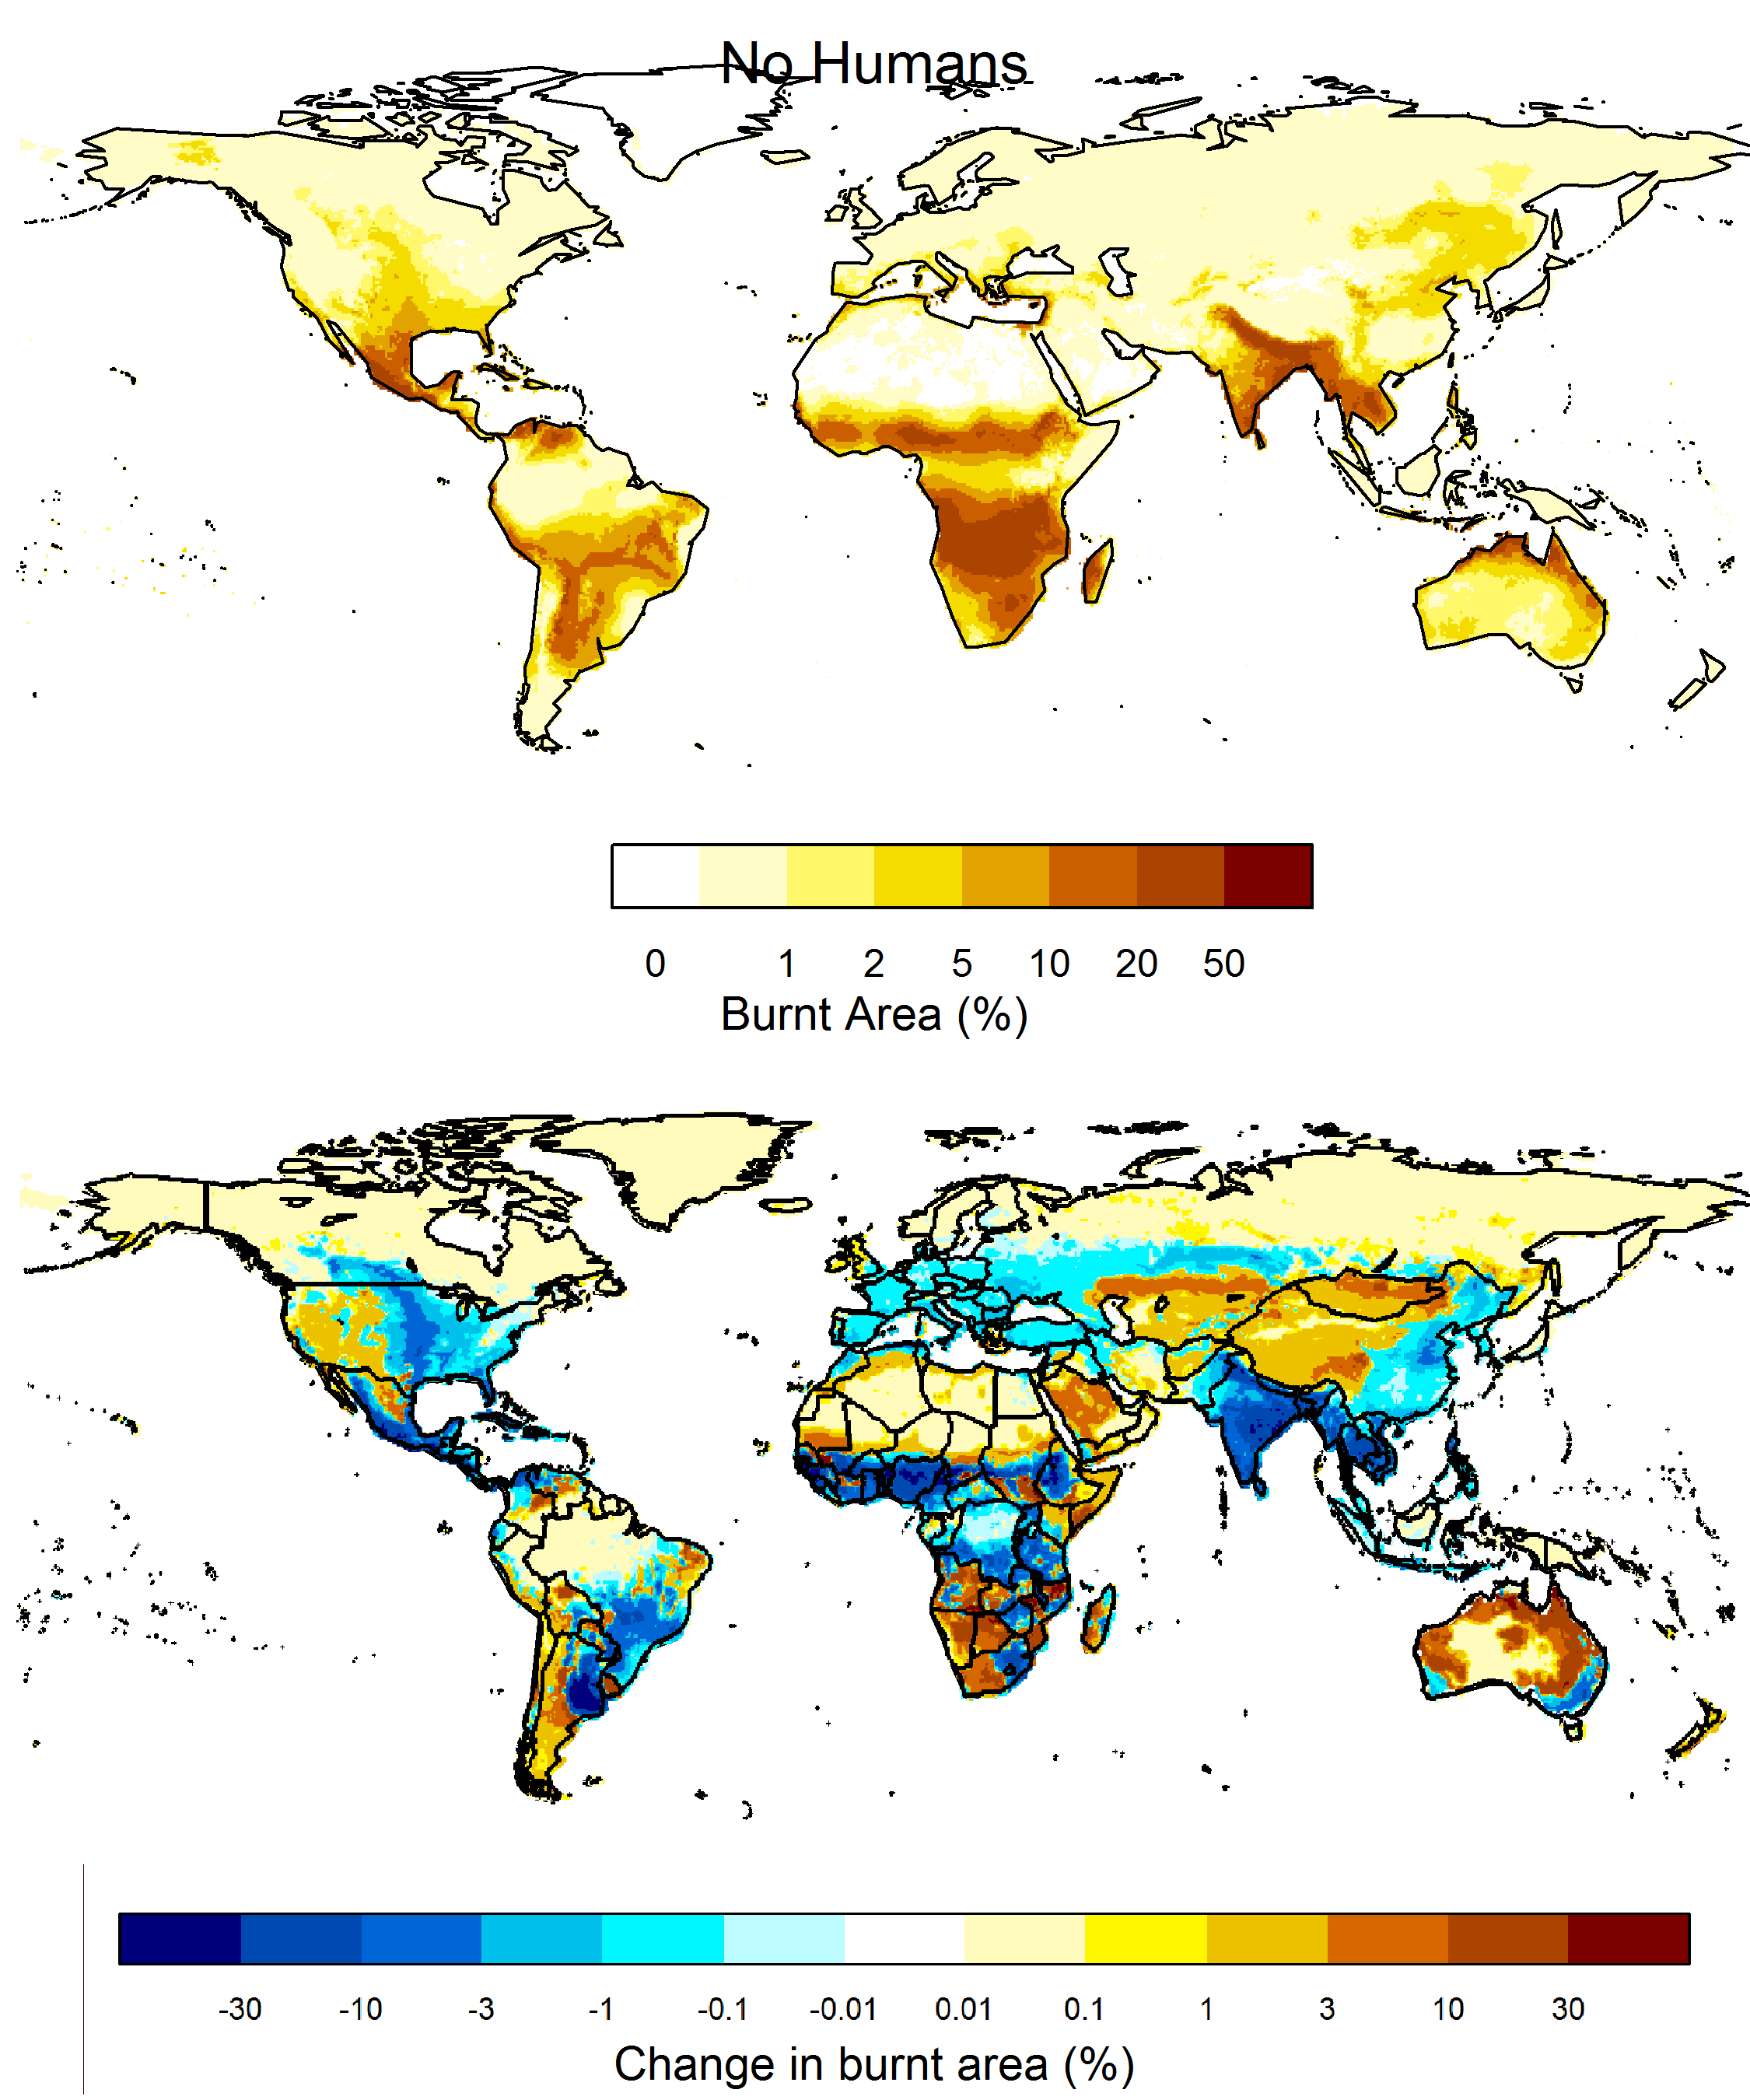
\includegraphics[trim={0 0 0 8cm},clip,width=6.5cm]{images/igntitions/IgntionInfoNoHumans}
    }
    \end{textblock*}
    %\visible<3->{
    %    \begin{tikzpicture}
    %        \node[anchor=south west,inner sep=0] (image) at (0,0) {
    %            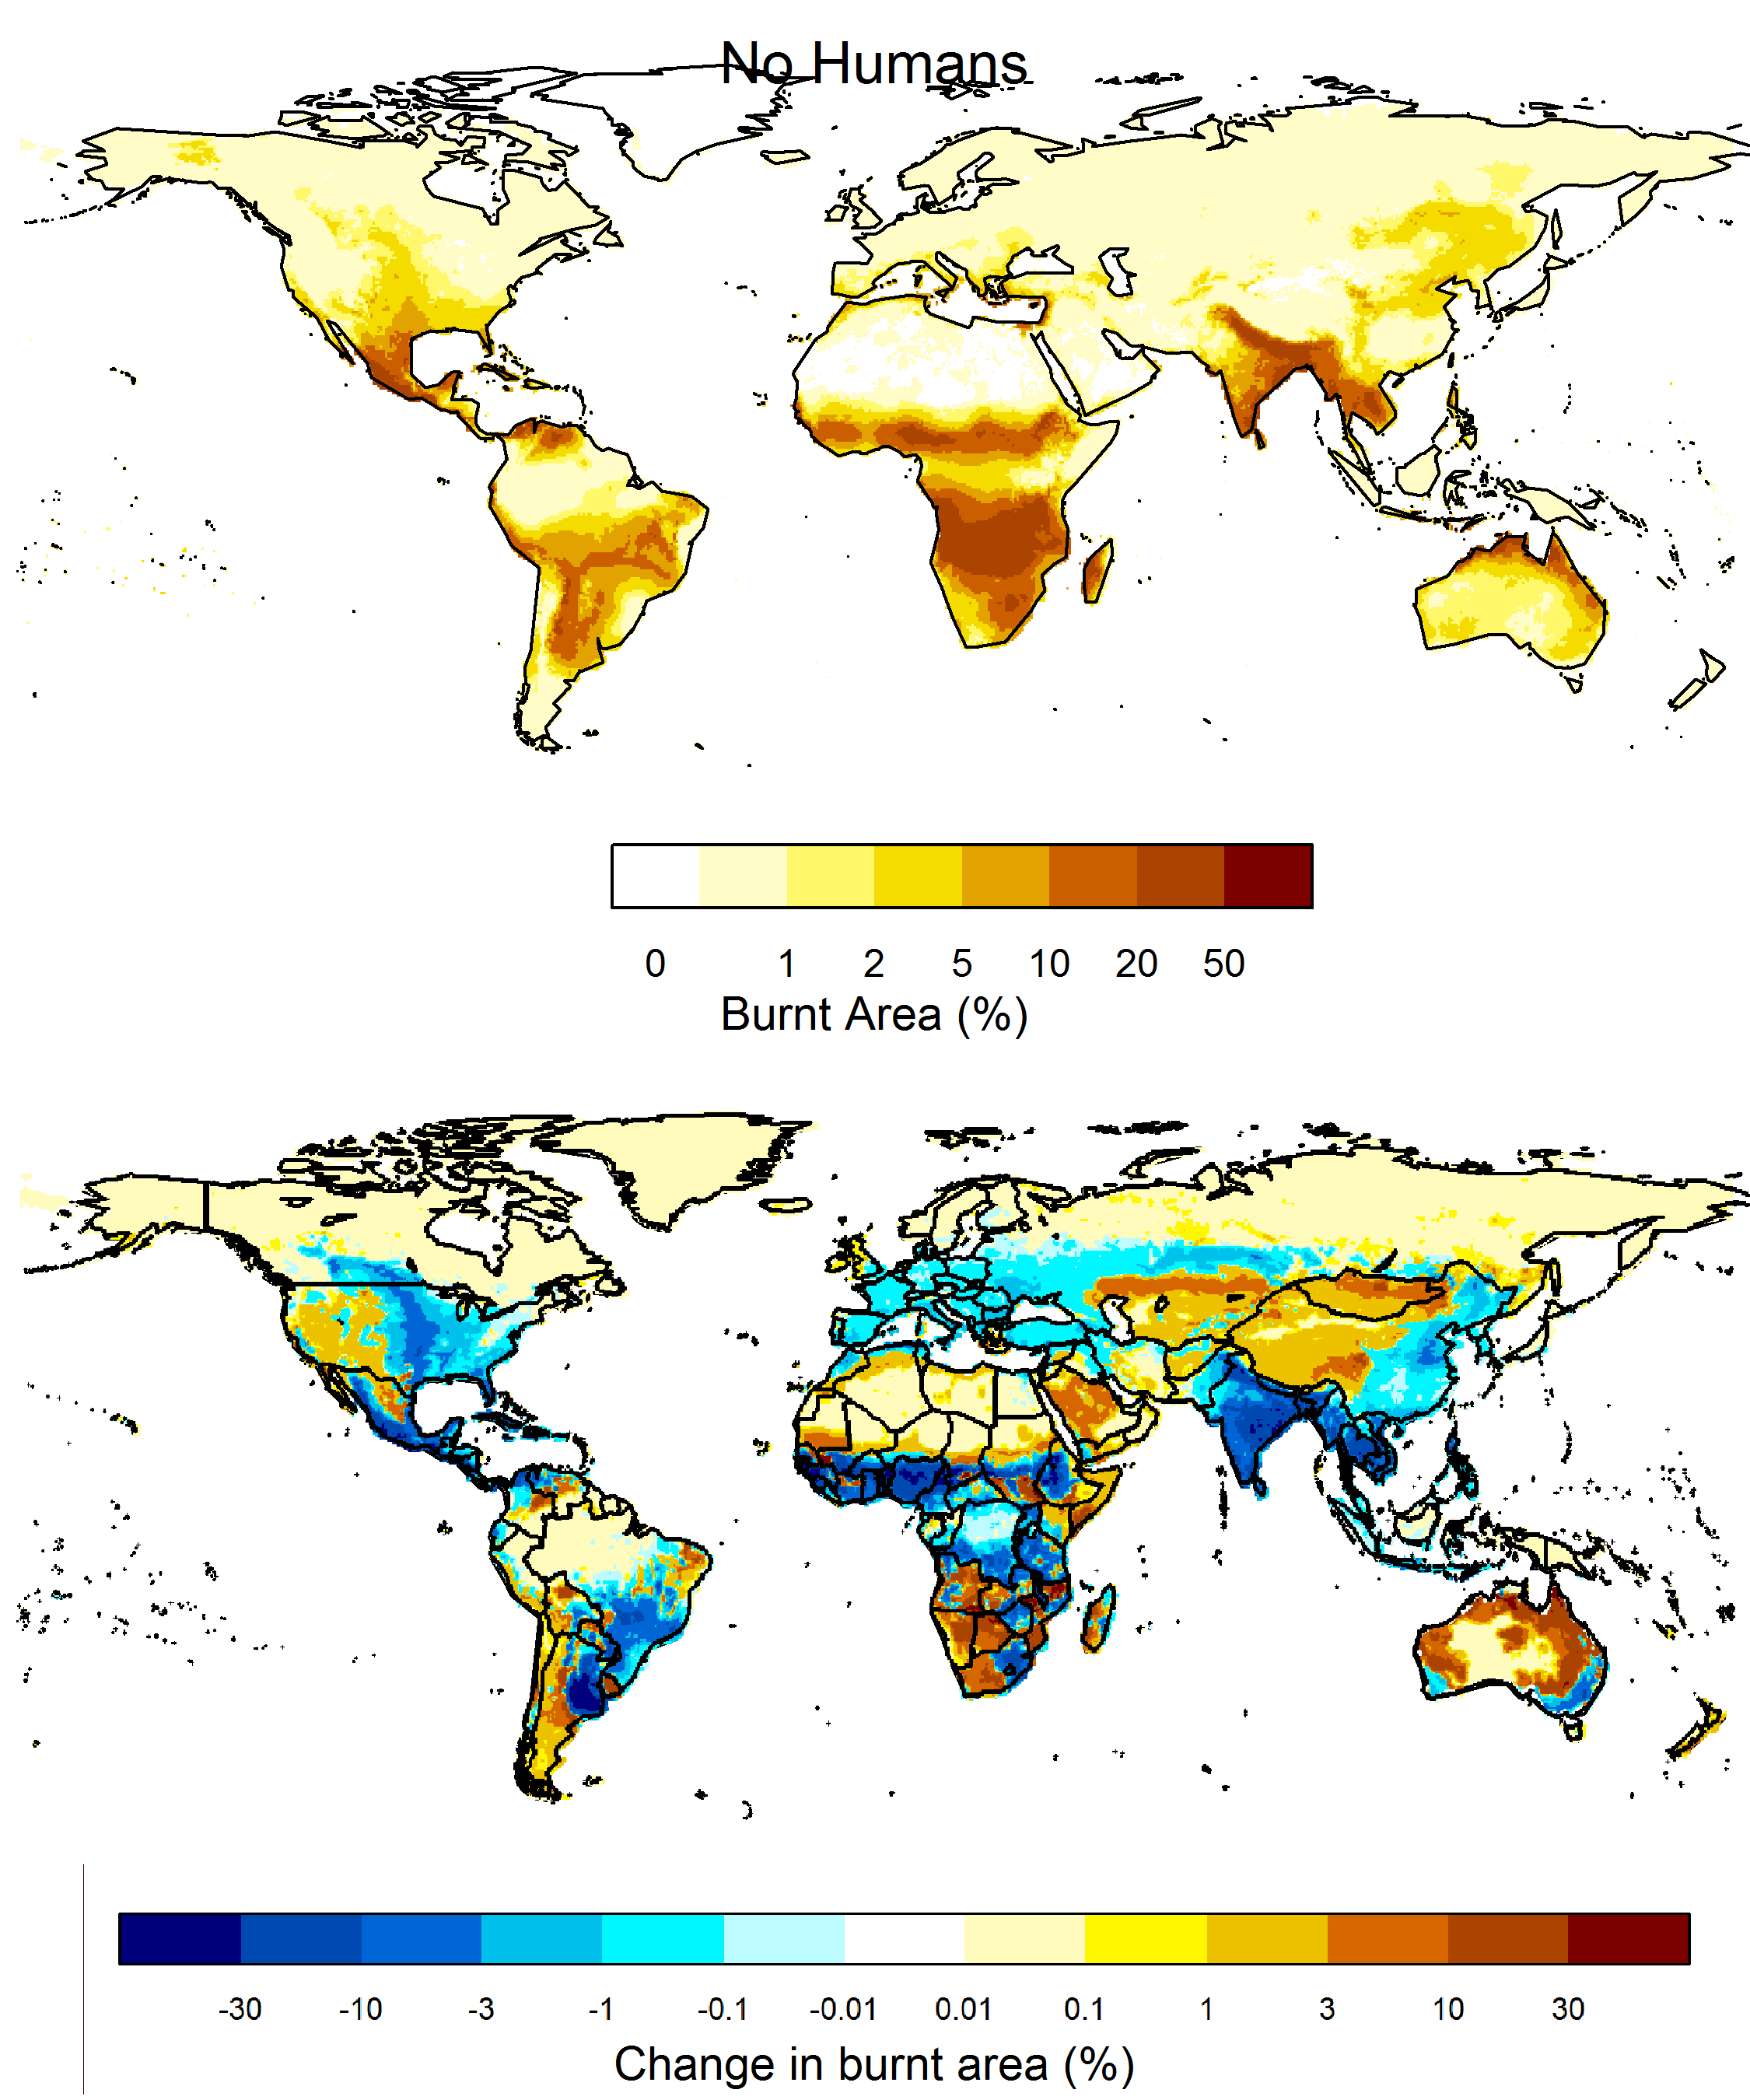
\includegraphics[trim={0 0 0 8cm},clip,width=11.0cm]{images/igntitions/IgntionInfoNoHumans}
    %        };
    %
            %\visible<-1> {\draw[white, fill = white] (5.5,4) -- (12.0,4) -- (12.0,0.0) -- (5.5,0.0) -- (5.5,4);}
    %    \end{tikzpicture}
    %}
\end{frame}

\pgfdeclareimage[width=1.0\paperwidth]{header-image}{header_images/firefighter}

\againframe<2-3>{controlMaps}

\begin{frame}
    \frametitle{Fire sensitivity}
\end{frame}
